\documentclass[tikz, border=5pt]{standalone}
\usetikzlibrary{shapes.callouts,calc,arrows,decorations.pathmorphing,intersections}
\tikzset{
  level/.style   = { thick, black }, %ultra thick
  connect/.style = { dotted, black },
  connect_vert/.style = { dashed, black },
  transition/.style={thick,black,->,>=stealth',shorten >=1pt},
  %notice/.style  = { draw, rectangle callout, callout relative pointer={#1} },
  %label/.style   = { text width=2cm }
}
\begin{document}
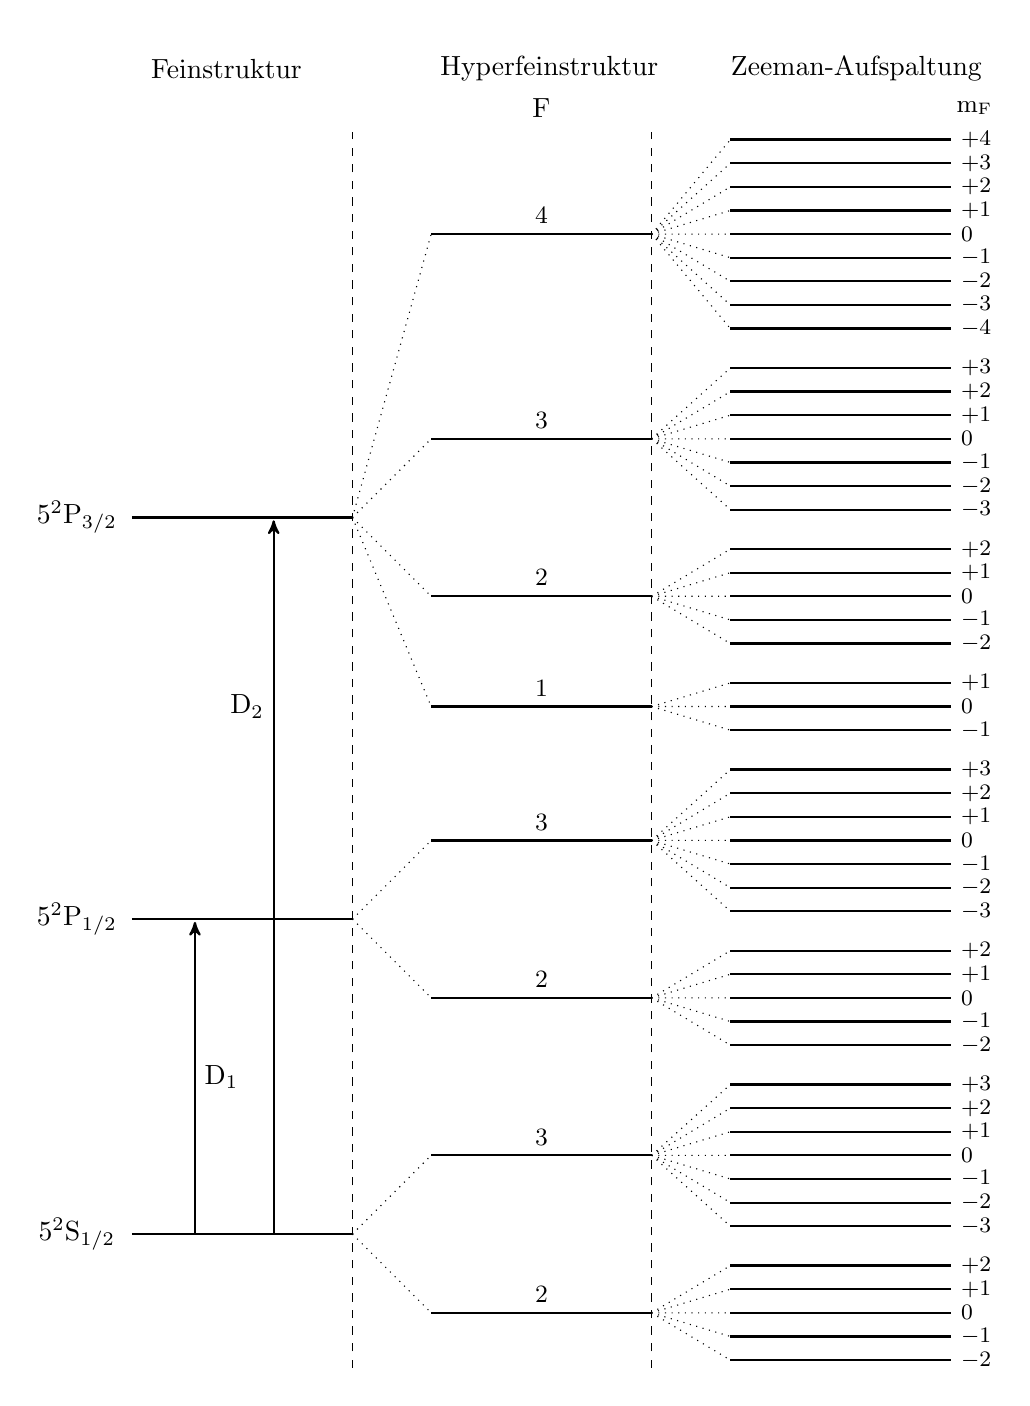
\begin{tikzpicture}
    % Draw all levels
    % Feinstrukur
    \draw[level] (0.2,1) -- (3,1);
    \draw[level] (0.2,5) -- (3,5);
    \draw[level] (0.2,10.1) -- (3,10.1);
  
    % Hyperfeinstruktur
    %s_1/2
    \draw[level] (4,0) -- node[above] {\small 2} (6.8,0);
    \draw[level] (4,2) -- node[above] {\small 3} (6.8,2);

    %p_1/2
    \draw[level] (4,4) -- node[above] {\small 2} (6.8,4);
    \draw[level] (4,6) -- node[above] {\small 3} (6.8,6);

    %p_3/2
    \draw[level] (4,7.7) -- node[above] {\small 1} (6.8,7.7);
    \draw[level] (4,9.1) -- node[above] {\small 2} (6.8,9.1);
    \draw[level] (4,11.1) -- node[above] {\small 3} (6.8,11.1);
    \draw[level] (4,13.7) -- node[above] {\small 4} (6.8,13.7);
    
    % Zeemanaufspaltung
    %s_1/2
    \draw[level] (7.8,-0.6) -- (10.6,-0.6) node[right] {\footnotesize $-2$};
    \draw[level] (7.8,-0.3) -- (10.6,-0.3) node[right] {\footnotesize $-1$};
    \draw[level] (7.8,0) -- (10.6,0) node[right] {\footnotesize $0$}; 
    \draw[level] (7.8,0.3) -- (10.6,0.3) node[right] {\footnotesize $+1$};
    \draw[level] (7.8,0.6) -- (10.6,0.6) node[right] {\footnotesize $+2$};

    \draw[level] (7.8,1.1) -- (10.6,1.1) node[right] {\footnotesize $-3$};
    \draw[level] (7.8,1.4) -- (10.6,1.4) node[right] {\footnotesize $-2$};
    \draw[level] (7.8,1.7) -- (10.6,1.7) node[right] {\footnotesize $-1$};
    \draw[level] (7.8,2) -- (10.6,2) node[right] {\footnotesize $0$}; 
    \draw[level] (7.8,2.3) -- (10.6,2.3) node[right] {\footnotesize $+1$};
    \draw[level] (7.8,2.6) -- (10.6,2.6) node[right] {\footnotesize $+2$};
    \draw[level] (7.8,2.9) -- (10.6,2.9) node[right] {\footnotesize $+3$};

    %p_1/2
    \draw[level] (7.8,3.4) -- (10.6,3.4) node[right] {\footnotesize $-2$};
    \draw[level] (7.8,3.7) -- (10.6,3.7) node[right] {\footnotesize $-1$};
    \draw[level] (7.8,4.0) -- (10.6,4.0) node[right] {\footnotesize $0$}; 
    \draw[level] (7.8,4.3) -- (10.6,4.3) node[right] {\footnotesize $+1$};
    \draw[level] (7.8,4.6) -- (10.6,4.6) node[right] {\footnotesize $+2$};

    \draw[level] (7.8,5.1) -- (10.6,5.1) node[right] {\footnotesize $-3$};
    \draw[level] (7.8,5.4) -- (10.6,5.4) node[right] {\footnotesize $-2$};
    \draw[level] (7.8,5.7) -- (10.6,5.7) node[right] {\footnotesize $-1$};
    \draw[level] (7.8,6) -- (10.6,6) node[right] {\footnotesize $0$}; 
    \draw[level] (7.8,6.3) -- (10.6,6.3) node[right] {\footnotesize $+1$};
    \draw[level] (7.8,6.6) -- (10.6,6.6) node[right] {\footnotesize $+2$};
    \draw[level] (7.8,6.9) -- (10.6,6.9) node[right] {\footnotesize $+3$};

    %p_3/2
    \draw[level] (7.8,7.4) -- (10.6,7.4) node[right] {\footnotesize $-1$};
    \draw[level] (7.8,7.7) -- (10.6,7.7) node[right] {\footnotesize $0$}; 
    \draw[level] (7.8,8) -- (10.6,8) node[right] {\footnotesize $+1$};

    \draw[level] (7.8,8.5) -- (10.6,8.5) node[right] {\footnotesize $-2$};
    \draw[level] (7.8,8.8) -- (10.6,8.8) node[right] {\footnotesize $-1$};
    \draw[level] (7.8,9.1) -- (10.6,9.1) node[right] {\footnotesize $0$}; 
    \draw[level] (7.8,9.4) -- (10.6,9.4) node[right] {\footnotesize $+1$};
    \draw[level] (7.8,9.7) -- (10.6,9.7) node[right] {\footnotesize $+2$};

    \draw[level] (7.8,10.2) -- (10.6,10.2) node[right] {\footnotesize $-3$};
    \draw[level] (7.8,10.5) -- (10.6,10.5) node[right] {\footnotesize $-2$};
    \draw[level] (7.8,10.8) -- (10.6,10.8) node[right] {\footnotesize $-1$};
    \draw[level] (7.8,11.1) -- (10.6,11.1) node[right] {\footnotesize $0$}; 
    \draw[level] (7.8,11.4) -- (10.6,11.4) node[right] {\footnotesize $+1$};
    \draw[level] (7.8,11.7) -- (10.6,11.7) node[right] {\footnotesize $+2$};
    \draw[level] (7.8,12) -- (10.6,12) node[right] {\footnotesize $+3$};

    \draw[level] (7.8,12.5) -- (10.6,12.5) node[right] {\footnotesize $-4$};
    \draw[level] (7.8,12.8) -- (10.6,12.8) node[right] {\footnotesize $-3$};
    \draw[level] (7.8,13.1) -- (10.6,13.1) node[right] {\footnotesize $-2$};
    \draw[level] (7.8,13.4) -- (10.6,13.4) node[right] {\footnotesize $-1$};
    \draw[level] (7.8,13.7) -- (10.6,13.7) node[right] {\footnotesize $0$}; 
    \draw[level] (7.8,14) -- (10.6,14) node[right] {\footnotesize $+1$};
    \draw[level] (7.8,14.3) -- (10.6,14.3) node[right] {\footnotesize $+2$};
    \draw[level] (7.8,14.6) -- (10.6,14.6) node[right] {\footnotesize $+3$};
    \draw[level] (7.8,14.9) -- (10.6,14.9) node[right] {\footnotesize $+4$};
    
    % connect levels
    %s_1/2
    \draw[connect] (6.8,0) -- (7.8,-0.6) (6.8,0) -- (7.8,-0.3) (6.8,0) -- (7.8,0) (6.8,0) -- (7.8,0.3) (6.8,0) -- (7.8,0.6);
    \draw[connect] (6.8,2) -- (7.8,1.1) (6.8,2) -- (7.8,1.4) (6.8,2) -- (7.8,1.7) (6.8,2) -- (7.8,2) (6.8,2) -- (7.8,2.3) (6.8,2) -- (7.8,2.6) (6.8,2) -- (7.8,2.9);
    \draw[connect] (3,1) -- (4,0) (3,1) -- (4,2);

    %p_1/2
    \draw[connect] (6.8,4) -- (7.8,3.4) (6.8,4) -- (7.8,3.7) (6.8,4) -- (7.8,4.0) (6.8,4) -- (7.8,4.3) (6.8,4) -- (7.8,4.6);
    \draw[connect] (6.8,6) -- (7.8,5.1) (6.8,6) -- (7.8,5.4) (6.8,6) -- (7.8,5.7) (6.8,6) -- (7.8,6) (6.8,6) -- (7.8,6.3) (6.8,6) -- (7.8,6.6) (6.8,6) -- (7.8,6.9);
    \draw[connect] (3,5) -- (4,4) (3,5) -- (4,6);

    %p_3/2
    \draw[connect] (6.8,7.7) -- (7.8,7.4) (6.8,7.7) -- (7.8,7.7) (6.8,7.7) -- (7.8,8);
    \draw[connect] (6.8,9.1) -- (7.8,8.5) (6.8,9.1) -- (7.8,8.8) (6.8,9.1) -- (7.8,9.1) (6.8,9.1) -- (7.8,9.4) (6.8,9.1) -- (7.8,9.7);
    \draw[connect] (6.8,11.1) -- (7.8,10.2) (6.8,11.1) -- (7.8,10.5) (6.8,11.1) -- (7.8,10.8) (6.8,11.1) -- (7.8,11.1) (6.8,11.1) -- (7.8,11.4) (6.8,11.1) -- (7.8,11.7) (6.8,11.1) -- (7.8,12);
    \draw[connect] (6.8,13.7) -- (7.8,12.5) (6.8,13.7) -- (7.8,12.8) (6.8,13.7) -- (7.8,13.1) (6.8,13.7) -- (7.8,13.4) (6.8,13.7) -- (7.8,13.7) (6.8,13.7) -- (7.8,14) (6.8,13.7) -- (7.8,14.3) (6.8,13.7) -- (7.8,14.6) (6.8,13.7) -- (7.8,14.9);
    \draw[connect] (3,10.1) -- (4,7.7) (3,10.1) -- (4,9.1) (3,10.1) -- (4,11.1) (3,10.1) -- (4,13.7);

    % Draw labels
    \node[label] at (1.4,15.8)  {Feinstruktur};
    \node[label] at (5.5,15.8)  {Hyperfeinstruktur};
    \node[label] at (5.4,15.3)  {F};
    \node[label] at (9.4,15.8) {Zeeman-Aufspaltung};
    \node[label] at (10.9,15.3)  {\small m\textsubscript{F}};

    \node[label] at (-0.5,1)  {5$^2$S$_{1/2}$};
    \node[label] at (-0.5,5)  {5$^2$P$_{1/2}$};
    \node[label] at (-0.5,10.1)  {5$^2$P$_{3/2}$};

    % vertical lines
    \draw[connect_vert] (3,-0.7) -- (3,15);
    \draw[connect_vert] (6.8,-0.7) -- (6.8,15);

    %transition
    \draw[transition] (1,1) -- (1,5);
    \draw[transition] (2,1) -- (2,10.1);

    \node[right] at (1,3) {D$_1$};
    \node[left] at (2,7.7) {D$_2$};
  
\end{tikzpicture}
\end{document}